\chapter{Solutions to $\NP$ problems}   %!% přejmenovat !!!
\label{chap:problems}

Since $\BPP$ is practically feasible even with classical computer, unlike $\NP$, it is reasonable to study feasibility of $\NP$ with DNA models. There is one big difference which enables DNA to be more powerful than classical computer which is extreme parallelism. Note that in one test tube there can be up to ... %!% najít a citovat
of DAE molecules. % Compared to one week performance of a supercomputer %!% udělat odhad !!!
Then if we assume some limit for input length so that probability of formation of certificate is reasonably high, $\NP$ can be feasible. % přepsat aby to šlo číst a dávalo to smysl ...
%!% pokud spustíme něco NP na PTM, máme extrémně malou pst výsledku, tady díky extrémní paralelizaci se můžeme dostat na rozumnou mez; zmínit proč nestuduju co-NP

First we define a simplifying model based on $\atam$ which was factically originally used by Winfree \cite{winfree_phd} as an example of a tilesystem solving $\sf HPP$ with DAE molecules. Then we use this model in few exaples of $\NP$ and $\NPC$ problems.

\section{Abstract model for DAE units}

In this section we will introduce a simplifying model for Winfree's solution to the $\mathsf{HPP}$. We have two reasons:
\begin{enumerate}   %!% opravdu to jsou ty důvody??
	\item the model will be based on the $\atam$ model,
	\item pictures will be easier-to-read.
\end{enumerate}

\begin{defn}   %!% uplně jinak !!!
	Let us define $\myatam$ (augmented $\atam$) as $\atam$ with one reduction and one augmentation:
	\begin{itemize}
		\item $\atam$ is reducted so that it only allows given glue-strengths for given tile-types defined in next point,
		\item augmented by $4$ other tile types from figure. %!% něco načmárat a refovat, spodní maj lepidla síly 2, ostatní 1 (krajní výjimka že ..)
	\end{itemize}
\end{defn}

\begin{remark}   %!% kam s tim?
	Those tiles with glue-strength $2$ will be used for generating random words. Note that these words can be restricted by arbitrary regular grammar rule.
\end{remark}

%!% popsat co znamená že je něco sestavitelný -- NP, že má něco pst sestavení -- BPP

Note those twice longer sticky ends on the bottom line.

In following examples this model will be set up to act similarly like $\NP$: $\exists y \; R(x,y)$. Although existence is not sure, it is very likely. Predicate $R$ will be ``enumerable in polynomial time'' for $x \in L$. In this context, {\em enumerable in polynomial time} will mean number of bindings, not number of biosteps. This can be assumed due to Turing universality of this model in $O(1)$ biosteps -- biostep complexity is not restrictive\footnote{From Turing's thesis, Turing machine is the most universal model.} and will be required to be $O(1)$ due to its lab complexity. On the other hand the binding complexity will be very important, we will be interested even in constants. This is because the less binding complexity, the less probability of error.

Note that the word on the bottom line can be restricted to belong to arbitrary regular language.

%!% odhady se dají zmenšit pomocí #E místo #V^2
%!% spodní řádek má 2x tak dlouhý lepidla !! vysvětlit proč

\begin{figure}[H]
\begin{center}
	\begin{subfigure}[b]{0.31\textwidth}
		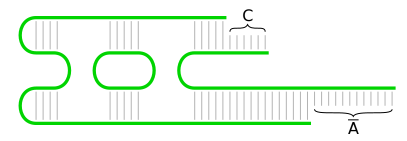
\includegraphics[width=\textwidth]{./figures/tile_model/DNA_struct.pdf} % 115mm
		\caption{Corner DAE unit}
		\label{fig:DNA_struct}
	\end{subfigure}
	\begin{subfigure}[b]{0.472\textwidth}
		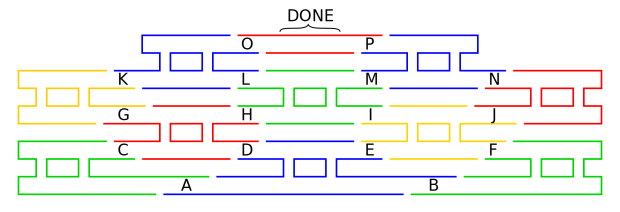
\includegraphics[width=\textwidth]{./figures/tile_model/DNA_assembly.pdf} % 175mm
		\caption{Scheme of self-assembly}
		\label{fig:DNA_assembly}
	\end{subfigure}
	\begin{subfigure}[b]{0.190\textwidth}
		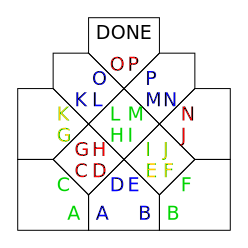
\includegraphics[width=\textwidth]{./figures/tile_model/abstract_model.pdf} % 70mm
		\caption{Abstract model}
		\label{fig:abstract_model}
	\end{subfigure}
	\caption{Evolution of $\myatam$ model from DAE units to tiles. Here glues {\sf A} and {\sf B} are of strength $2$.}
	\label{fig:evolution}
\end{center}
\end{figure}

\subsection{Feasibility of the class $\BPP$}
	
	As it is often conjectured that the class $\P$ is the class of somehow practically feasible problems, here we introduce similar conjecture for feasible DNA algorithms. The corresponding debate can be found in \cite{book_comp}. %!% najít a citovat delší filozofickou rozpravu
	
	\begin{conj}   %!% conjecture nebo lépe?
		Feasible DNA algorithms comply $Bs(n)\in O(1)$; $Bnd(n),\,Ti(n),\,Gl(n)\in \P$.   %!% možná postačí pro poly algoritmus mín jak \P tile a glue !!! ale spíš ne
	\end{conj}
	
	\begin{thm}   %!% tohle je potřeba někde najít a citovat
		Probabilistic Turing machine can be simulated by probabilistic cellular automaton.
	\end{thm}
	
	\begin{proof}
		Can be found in \ldots
	\end{proof}
	
	\begin{thm}   %!% nějak pojmenovat model, deterministic version by Winfree
		$\myatam$ can simulate probabilistic cellular automaton.
	\end{thm}
	
	\begin{proof}
		Blabla. % poměrem částeček umim nastavit pravděpodobnosti, zbytek důkazu Winfree
	\end{proof}
	
	\begin{cor}
		$\BPP$ is decidable by $\myatam$.
	\end{cor}
	
	%!% nák rozumně vysvětlit že \NP se dá na PTM docela dobře spočítat
	% The model can practically handle also $\NP$ languages (not theoretically, of course) because 

\section{Graph 3-coloring}

Remind original Knuth's algorithm at \url{http://www.iti.fh-flensburg.de/lang/algorithmen/sortieren/networks/oetsen.htm}! And prove that everything goes fine! Robusticity? %!% citovat někde

First idea: Generate all bonds with colored atoms and check the entire system (haha, complexity like $O(n^4)$ because $|E| \in O(n^2) $). Second solution: Generate a reverse-order sequence of vertices and let it order in the correct order. All pairs should meet each other, the problem to solve is whether all pairs really meet each other. After that check that the area is full like Winfree -- from one side to the other. Improvement: the check can be triggered from both sides simultaneously.

\subsection*{Set of tiles}

First of all the graph needs to have even number of vertices, thus one separated non-colored vertex has to be added if applicable. Then follow these rules which are showed in an example, see Figure \ref{fig:3-color}.
\begin{description}
	\item[Bottom line] For every pair $(2k,\,2k+1)$ there will be a bottom-type tile with non-colored numbers $(2k+2,\,2k)$ on the bottom and with all feasible\footnote{If $(2k+1,\,2k)$ are connected, same-colored numbers are omitted.} color combinations of $(2k+1,\,2k)$ on the top. From practical decoding reasons (see Winfree \cite{winfree_phd}) the sequences encoding colored numbers on the top must be physically present also wherever on the bottom DNA strand, see Figure \ref{fig:bottom_tile}. $\frac{9n}{2}$ tile types were required.
	\item[Bottom corner tiles] Both corner tiles are connected on the bottom by the highest and the lowest non-colored number, respectively, and have their special glue (\# for $-\infty$ and * for $+\infty$, respectively) on the top. These first two sets of tiles generate all colorings of given graph (without those omitted in previous step) with reverse order of numbers. $2$ tile types were required.
	\item[Inner tiles] These tiles are responsible for ordering\footnote{Principially they are the same as in Winfree \cite{winfree_phd}.}. There exist all color combinations for all different numbers with two important exceptions. There {\em do not} exist tiles with numbers of connected vertices with the same color. Thus, as soon as there appears such forbidden combination, the self assembly cannot continue and reach ``DONE''. Because the numbers are generated in reverse order they must meet each other -- note that they simply cannot ``jump'' and every number has to exchange with all the higher ones as well as with the lower ones. This implies that every forbidden combination would be revealed, thus it answers correctly if and only if the coloring is correct. The second exception are those described in the following paragraph. $9n^2$ tile types were required.
	\item[Border tiles] There are two tile types on the borders, one with sharp, one with asterisk. They keep the structure growing up.
	\item[Checking tiles] As soon as the biggest and the smallest number reach * and \#, respectively, there are two special tiles which start checking whether nothing is missing. Note that all tiles had time enough to get into correct order. In this setup checking tiles do not need to check correct order thus there can exist only two types of checking sequences ``C'' and ``D'' with all color-number combinations of middle numbers -- ``D'' with the smaller half, ``C'' with the higher half. $3n$ tile types were required.
	\item[DONE tile] If everything is checked and checking sequences meet each other, ``DONE'' tile will be connected to signalize correct solution. $1$ tile type was required.
\end{description}
\begin{figure}[H]
\begin{center}
	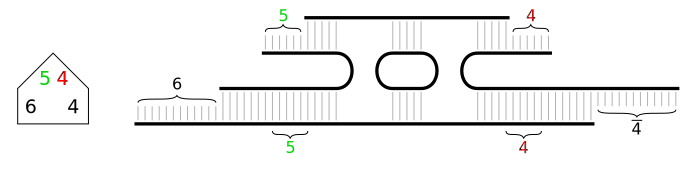
\includegraphics[scale=0.75]{./figures/3-color/bottom_tile.pdf}
	\caption{Bottom tile with desired sequences in the bottom strand.}
	\label{fig:bottom_tile}
\end{center}
\end{figure}
Summed up, this DNA algorithm requires $9n^2$ tile types. Glue complexity is ...

The first idea's binding complexity was like $O(n^4)$, the second is already $O(n^2)$, the binding complexity is $1\nicefrac{1}{2}\;n^2$. The improvement decreases it to $1\nicefrac{1}{4}\;n^2$.

\begin{figure}[H]
\begin{center}
	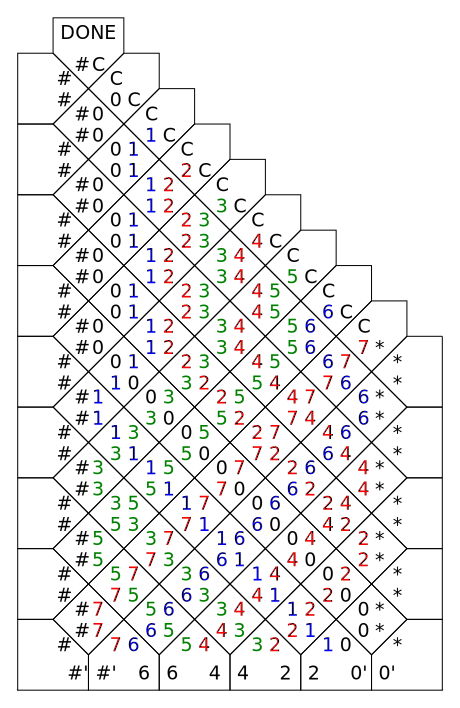
\includegraphics[scale=0.75]{./figures/3-color/3-color.pdf}
	\caption{3-color computation.}
	\label{fig:3-color}
\end{center}
\end{figure}


\newpage
\input{./include/2-results_3-isomorph.tex}

\newpage
\section{$k$-clique}

%!% rozmyslet a překopat:

$k$-clique problem belongs to $\NP$-complete problems. Note that $k$-clique problem in $G$ is equivalent to $k$-independent set in $\overline{G}$ and that is equivalent to $n-k$-vertex cover of $\overline{G}$ so we can assume $k \leq \frac{n}{2}$. Like before we add an unchecked vertex if $k$ is odd so we will assume $k$ to be even. % možná: and there exists a DNA system with very low complexity: $\min\bigl\{ 1\nicefrac{1}{4}\;\bigl( \frac{n}{2} \bigr) ^2 ,\; 1\nicefrac{1}{4}\;k^2 \bigr\}$.

\subsection*{Set of tiles}

\begin{description}
	\item[Bottom line] For now there are tiles with $2l-2$ and $2l$ ($0 < l \leq \frac{k}{2}$) on the bottom and with an arbitraty ordered\footnote{Note that this restriction does not reduce the set of possible $k$-member subsets.} pair of different numbers from $1$ to $n$ with $k-2l+2$-th and $k-2l+1$-th colors, respectively, on the top. Note that now the order of colors is given and do not forget that they should also contain those upper sequences once more on the bottom strand. $\frac{kn^2}{4}$ tile types were required. % na prvních místech nejnižší čísla, na nejvyšších ty nejvyšší -> sníží počet dlaždic ale je s tim sraního
	\item[Bottom corner tiles] Are exactly the same. $2$ tile types were required.
	\item[Inner tiles] These tiles are now responsible for ordering by color during which they check existence of {\em every} edge in similar manner to previous problems. And because the first line contains them in reverse order there will meet each other. $k^2 n^2$ tile types were required. % $k^2 \cdot 2#E $
	\item[Border tiles] These tiles are exactly the same like for 3-coloring.
	\item[Checking tiles] As soon as the most left color reaches sharp and the most right color reaches asterisk, checking is triggered in similar manner to 3-coloring. $kn$ tile types were required.
	\item[DONE tile] This is exactly the same like 3-coloring. $1$ tile type was required.
\end{description}
Summed up, this DNA algorithm requires $k^2 n^2$ tile types. Binding complexity is $1\nicefrac{1}{4}\;\min\{k^2,\,(n-k)^2\}$ Glue complexity is ... % $k^2 \cdot 2#E $

\begin{figure}[H]
\begin{center}
	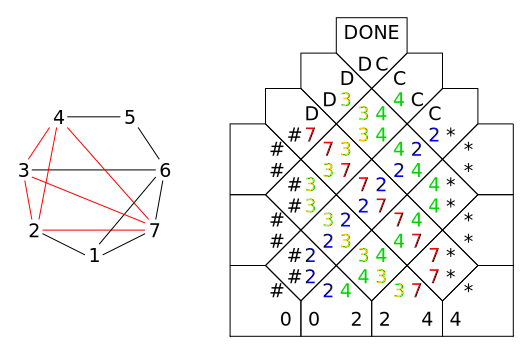
\includegraphics[scale=0.75]{./figures/k-clique/k-clique.pdf}
	\caption{$k$-clique computation. Color order is defined by their wavelength.}
	\label{fig:graph_iso}
\end{center}
\end{figure}


